\documentclass[pdftex,12pt,a4paper]{article} 
% margin size
\usepackage[margin=1in]{geometry}

% Math and algorithms
\usepackage{amsmath,amssymb,amsthm,esint}  % For both in-line and equation mode
\usepackage{bbm}
\usepackage{bm}
\usepackage{algorithm}
\usepackage{algorithmic} % Algorithm styles, need to be nested for the example shown
\usepackage{aliascnt}
\numberwithin{equation}{section} % Numbering of our equations per section
\newtheorem{theorem}{Theorem}
\newtheorem{definition}{Definition}
\newtheorem{proposition}{Proposition}
\newtheorem{corollary}{Corollary}
\newtheorem{remark}{Remark}

\usepackage{setspace} %Spacing on the front page for crest and titles
\usepackage[]{fncychap} % Styles can be Sonny, Lenny, Glenn, Conny, Rejne, Bjarne and Bjornstrup
\usepackage[hyphens]{url} % Deals with hyphens in urls to make them clickable
\usepackage{xcolor} % Great if you want coloured text

% Figures
\usepackage{graphicx} % Inserting images
\graphicspath{ {../figures/} } 

% Tables
\usepackage{tabularx}
\usepackage{multirow} 
\renewcommand{\arraystretch}{1.5}

% Appendix
\usepackage{appendix} 

\usepackage{natbib}
\usepackage{comment}

% Tikz figures
\usepackage{tikz}
\newcommand{\ImageWidth}{14cm} 
\usetikzlibrary{decorations.pathreplacing,positioning, arrows.meta} 

% Fancy headers and footnotes
\usepackage{fancyhdr}
\usepackage[symbol]{footmisc}
\renewcommand{\thefootnote}{\fnsymbol{footnote}} 

% Hyperlinks and auto-references
\usepackage[hidelinks]{hyperref}  
\def\sectionautorefname{Section}
\def\appendixname{Appendix}
\newcommand{\propositionautorefname}{Proposition}
\newcommand{\definitionautorefname}{Definition}
\newcommand{\corollaryautorefname}{Corollary}  

\setlength{\footnotesep}{0.5cm}
%%%%%%%%%%%%%%%%%%%%%%%%%% DOCUMENT STARTS %%%%%%%%%%%%%%%%%%%%%%%%%%%%% 

\begin{document} 
% Front page 
%\pagestyle{empty} 

% Warwick Crest
\begin{center}
	\includegraphics[scale = 0.5]{preamble/warwick-crest.pdf} 
\end{center}
\vspace{5mm}

% Dissertation Title
\begin{center}
	\textbf{\begin{huge}
		Swiping Left and Right:\\
	\end{huge}}
	\vspace{3mm}
	\textbf{\begin{huge}
		Two-Sided Search in Swipe-Based Dating Platforms 
	\end{huge}} 
	\vspace{8mm}
\end{center}

% Author
\begin{center}
	\textbf{\large Patricio Hernandez Senosiain\footnote[1]{I am immensely grateful to Dr. Jonathan Cave for his supervision throughout the course of this project, during which he provided invaluable advice, support, and numerous stimulating discussions.}}
	
\end{center}

% Supervisor, Department and Date
\begin{center}
	%{\large Supervisor: Dr. Jonathan Cave}\\
	%\vspace{5mm}
	\textbf{\large Department of Economics}\\ 
	{\large April 2022\\}
	\vspace{10mm}
\end{center} 

% Abstract
\begin{center}
	%\section*{Abstract}
%\addcontentsline{toc}{section}{Abstract} 
\begin{abstract}
    \noindent In today's love market, swipe-based dating platforms (SBDPs) such as Tinder or Bumble have a well-established presence, but novel platform features can add significant complexities to the user's search problem in ways that have been largely under-studied in existing literature.
    This paper formulates a model of two-sided search within SBDPs, where agents with heterogeneous preferences seek multiple romantic partners whilst facing intertemporal action constraints.
    Using numerical methods, I approximate stationary equilibria and perform comparative statics on various exogenous parameters that help explain stylised empirical facts.
    Finally, agent-based simulations are used to asses the structure of stationary equilibria as well as its attainability under myopic best-response dynamics.  
    \vspace{1cm}\\
    \noindent\textbf{Keywords:} Optimal Search, Two Sided Matching, Agent-Based Modeling\\
    %\vspace{0in}\\
    \noindent\textbf{JEL Codes:} C78, D83, C63\\
    \bigskip
\end{abstract} 
\end{center} 
\vspace{5mm}




  
\title{Why Do Men Keep Swiping Right? Two-Sided Search in Swipe-Based Dating Platforms\thanks{Contact: \href{mailto:hdzsen.patricio@gmail.com}{hdzsen.patricio@gmail.com}. All code produced for this project and the most recent version of this paper is available under GitHub repository \href{https://github.com/patohdzs/project-swipe}{\texttt{patohdzs/project-swipe}}. The author is grateful to Dr. Jonathan Cave for his excellent supervision throughout the course of this project, during which he provided invaluable advice and support.}} 
\author{Patricio Hernandez Senosiain}  
\date{\today}

\maketitle
%\section*{Abstract}
%\addcontentsline{toc}{section}{Abstract} 
\begin{abstract}
    \noindent In today's love market, swipe-based dating platforms (SBDPs) such as Tinder or Bumble have a well-established presence, but novel platform features can add significant complexities to the user's search problem in ways that have been largely under-studied in existing literature.
    This paper formulates a model of two-sided search within SBDPs, where agents with heterogeneous preferences seek multiple romantic partners whilst facing intertemporal action constraints.
    Using numerical methods, I approximate stationary equilibria and perform comparative statics on various exogenous parameters that help explain stylised empirical facts.
    Finally, agent-based simulations are used to asses the structure of stationary equilibria as well as its attainability under myopic best-response dynamics.  
    \vspace{1cm}\\
    \noindent\textbf{Keywords:} Optimal Search, Two Sided Matching, Agent-Based Modeling\\
    %\vspace{0in}\\
    \noindent\textbf{JEL Codes:} C78, D83, C63\\
    \bigskip
\end{abstract}  
\setcounter{page}{0}
\thispagestyle{empty} 

\clearpage
\renewcommand{\thefootnote}{\arabic{footnote}}
\pagestyle{fancy}
\fancyhf{}
\setlength{\headheight}{14.49998pt}
\addtolength{\topmargin}{-2.49998pt} 
\lhead{Why Do Men Keep Swiping Right?}
\def\layersep{2.5cm}
\pagenumbering{arabic}
\lfoot{\centering \thepage}
\onehalfspacing   

% Sections
\section{Introduction}
\label{sec:Introduction} 
%To make a call to the introduction, put \ref{sec:Introduction} 
\textbf{Points to discuss on introduction}
\begin{itemize}
    \item What is Tinder?
    \begin{itemize}
        \item When was it started?
        \item What is swiping?
        \item How popular it is?
    \end{itemize}
    \item Why does Tinder pose an interesting economic problem?
    \begin{itemize}
        \item Stage interaction
        \item Platform features: budgets, observability, directed search, asynchronicity
        \item Repeated games: curse of dimensionality, beliefs and meta-beliefs
    \end{itemize}
    \item What does this paper study?
    \begin{itemize}
        \item Model of two-sided search with strategic considerations
        \item Equilibrium refinement, computation, and analysis
        \item Planner considerations on directed search and budget setting
    \end{itemize}
    \item What does this paper contribute?
    \begin{itemize}
        \item First model to address budgeted search in Tinder?
        \item First model to combine idiosyncracy and pizzaz
        \item Case study for the use of computational techniques in 
    \end{itemize}
\end{itemize}
\subsection{Related Work}
\begin{itemize}
    \item Searching and Matching
    \begin{itemize}
        \item Gale-Shapley, Roth\&Sotomayor
        \item Two-sided: \cite{burdett1998two}, \cite{chade2006matching}, Smith, Adachi
    \end{itemize}
    \item Mean-Field Game Theory: \cite{iyer2014mean}, \cite{gummadi2013optimal}, \cite{jovanovic1988anonymous}
    \item Modern Dating Apps: \cite{olmeda2021towards}, \cite{kanoria2021facilitating}
\end{itemize}
\section{Theoretical Model}
\label{sec: model}
\subsection{Setup} 
Consider the two-sided search market formed by the Tinder platform with both male and female agents looking for potential partners. For ease of exposition, I assume that this market is heteronormative such that male agents search exclusively for female agents and vice-versa. Time is discrete and indexed $t=0,1,...$ over an infinite horizon. At every time period, agents from each sex are paired up and presented a suggested partner from the opposite side of the market. Each agent has an attractiveness type $\theta \in \Theta := [0,1]$ which is unknown to them but observable to their suggestion, and it is common knowledge that this is the case. After being paired, agents observe the suggested partner's attractiveness and can then choose whether to swipe left (dislike) or right (like) on their suggestion, yielding an action space of $\mathcal{A}=\{ \text{left},\; \text{right}\}$. If both agents swipe right on one another, they are said to have \textit{matched} and both receive a matching payoff, however, if either agent swipes left, they both receive a payoff of zero. Contingent on swiping right on a suggestion of attractiveness $\theta$, a user earns a matching payoff $u(\theta)$, where $u(\cdot)$ is a strictly increasing, concave function that satisfies $u(0) = 0$. This last property stems from the fact that, in Tinder, users are allowed to unmatch with each other, thus implying that matching with the least attractive individual on the other side of the market is weakly preferred to not matching. After payoffs have been received, players are then paired with a different suggestion and the above stage interaction is repeated. Given the large number of agents in SBDA platforms, I assume that agents are paired \textit{anonymously} in the style of \cite{jovanovic1988anonymous}, thus abstracting from history-related complexities. Furthermore, to the agents' knowledge, pairings are decided in an unknown manner (since SBDA's are generally secretive regarding the algorithms used), effectively making their problem on of random search.

Considering the above, it is evident that swiping right in the stage interaction is both weakly dominant for all agents and yields a Pareto-optimal outcome, thus implying that, in a repeated interaction, the market equilibrium would have all agents exclusively swiping right. Since that the main selling point of SBDA's is a reduction in searching costs, which is accomplished when matches have a high likelihood of resulting in real-life romantic attraction, Tinder places a cap on the total number of right swipes for each user, thus making it a form of costly signalling. I refer to the total number of right-swipes a user has left as its \textit{budget}, $b_t$, which evolves dynamically according to the law of motion:
$$
  b_{t+1}= b_{t}- a_{t}
$$
where the starting budgets for each sex, $B_m$ and $B_w$, are determined exogenously. The budget sets for men and women are thus defined by $\mathcal{B}_{i}=\{b \in \mathbb{Z} : 0\leq b \geq B_i\}$, with $i=m,W$ respectively. Each period, $\lambda_m$ new men and $\lambda_w$ new women enter the platform, with their attractiveness drawn i.i.d from distributions with cumulative distribution functions $F_m$ and $F_w$, respectively. Importantly, agents depart from the platform in one of two ways: they can leave \textit{endogenously}, if they expend their swiping budget, or \textit{exogenously} with probability $(1-\delta)$. This admits to the interpretation of a geometrically distributed lifetime within the platform, parametrized by $\delta$, and implies that users use this as a discounting factor for future payments.

\begin{figure}[ht]
    \centering
        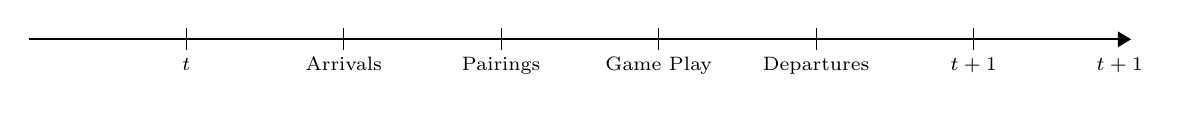
\begin{tikzpicture}
            % draw horizontal line   
        \draw[thick, -Triangle] (0,0) -- (\ImageWidth,0) node[font=\scriptsize,below left=3pt and -8pt]{$t+1$};

        % draw vertical lines
        \foreach \x in {1,2,...,6}
        \draw (\x*2 cm,4pt) -- (\x*2 cm,-4pt);

        \foreach \x/\descr in {2/t, 4/\text{Arrivals}, 6/\text{Pairings}, 8/\text{Game Play}, 10/\text{Departures}, 12/t+1}
        \node[font=\scriptsize, text height=1.75ex,
        text depth=.5ex] at (\x,-.3) {$\descr$}; 

        % braces
        %\draw [thick ,decorate,decoration={brace,amplitude=5pt}] (4,0.7)  -- +(2,0) 
        %    node [black,midway,above=4pt, font=\scriptsize] {Training period};

        %\draw [thick,decorate,decoration={brace,amplitude=5pt}] (6,-.9) -- +(-1,0)
        %    node [black,midway,font=\scriptsize, below=4pt] {Testing period};  
    \end{tikzpicture}
    \caption{Sequence of events within each time period} \label{fig:timeline}
\end{figure}

Given the above, a number of simplifications to the explored setting are possible. 

- 1. An agent’s decision on any given time period depends fundamentally on the attractiveness of the suggested partner and their own budget

I restrict attention to stationary Markov strategies, defined by $\sigma_m: \Theta \times\mathcal{B}_m\rightarrow \Delta\mathcal{A}_m$ for men and $\sigma_w:\Theta \times\mathcal{B}_w\rightarrow \Delta\mathcal{A}_w$ for women, where $\Delta S$ denotes the probability simplex over set S. 

\subsection{The Dating Market}
Given the sequence of events described in the stage interaction above, I now outline the aggregate market variables that make up the Tinder market, as these must be considered within the model given their endogenous relation with strategic search behaviour. At any given time $t$, the masses of men and women on Tinder are denoted by $N_{mt}$ and $N_{wt}$, respectively. Furthermore, let $\pi_{it}:\mathcal{B}_{i}\rightarrow[0,1], \quad i=m,w$ be the probability mass function over agent budgets. These are endogenously determined since the flow of agents into lower budget levels and eventually out of the platform depends on their swiping decisions. All in all, by considering aggregate variables on both sides of the platform, the Tinder market at time period $t$ is defined as $\Psi_t=(N_{mt},N_{wt},\pi_{mt},\pi_{wt})$. Finally, since gender imbalances can exist, resulting with unpaired agents in the long side of the market, a pairings process must be fixed. Given fairness considerations as well the efficient, automated nature of SBDA platforms, this paper assumes a frictionless matching technology, and models pairings as a Bernoulli process parametrized by market tightness, ie. the probability of receiving a suggestion on each side:
$$
\tau_t=\min \Big\{\frac{N_{wt}}{N_{mt}} ,1 \Big\} 
$$

For most of this paper, I focus on characterizing user behaviour and its resulting implications in a stationary setting, although some discussion of coupled strategy and market dynamics is provided in \textbf{Section 4}. Given this, it is firstly important to characterize the market steady state, which again arises as a result of exogenous pairing and departure processes as well as endogenous search behaviour. When doing so, time subscripts are omitted, thus denoting the steady state as the Tinder market $\Psi(\sigma)=(N_m(\sigma),N_w(\sigma),\pi_m(\cdot \,|\, \sigma),\pi_w(\cdot \,|\, \sigma))$ such that $\Psi_t(\sigma)=\Psi_{t+1}(\sigma)=...=\Psi(\sigma)$. This market steady state must satisfy the balanced flow equations. Firstly, the entry flow of agents into the platform must equal the departure flow, thus for $i=m,w$: 

% Budget dist equations
\begin{equation} 
    \lambda_i \;=\; \underbrace{N_i(1-\delta)}_{\text{Exogenous Deaths}} + \underbrace{N_i \pi_i(1) \delta \tau_i \int_{\Theta}\sigma_i(\theta,1)\,dF_{j}(\theta)}_{\text{Expended Budgets}} 
\end{equation} 

Secondly, the flow of agents into any particular budget level must equal the outflow of agents from that same level: 

\begin{equation}
    \underbrace{N_i \pi_i(b+1) \delta \tau_i \int_{\Theta} \sigma_i(\theta,b+1)\,dF_{j}(\theta)}_{\text{Inflow into $b$}} \;=\; \underbrace{N_i \pi_i(b) (1-\delta) + N_i \pi_i(b) \delta \tau_i \int_{\Theta} \sigma_i(\theta,b)\,dF_{j}(\theta)}_{\text{Outflow from $b$}}
\end{equation}

Finally, the entry flow of agents into the platform must equal the outflow from the top budget level:

\begin{equation}
    \lambda_i \;=\; \underbrace{N_i \pi_i(B_i)(1-\delta)}_{\text{Exogenous outflow from B}} + \underbrace{N_i \pi_i(B_i)\delta \int_{\Theta} \sigma_i(\theta,b)\,dF_{j}(\theta)}_{\text{Endogenous outflow from B}}
\end{equation}


% Original eqs
\begin{comment}
\begin{equation} 
    \underbrace{\lambda_m \Big( F_m(\theta'')-F_m(\theta') \Big)}_{\text{Entering Agents}}\;=\;\underbrace{(1-\delta)N^m(\sigma)}_{\text{Exogenous Deaths}}+\quad  \underbrace{\delta N^m(\sigma)  G^m_b(1 \,|\, \sigma)\int_{\Theta}\sigma_m(\theta,1)\,dG^w_\theta(\theta \,|\, \sigma)}_{\text{Expended Budgets}} 
\end{equation} 

\begin{equation}
    \underbrace{\left(\delta  \int_{\Theta}\sigma_m(\theta,b+1)\,dw_\theta(\theta \,|\, \sigma)\right)N_mR^m_{b+1}}_{\text{Transitions into budget b}}\;=\;\underbrace{\left((1-\delta)+\delta \int_{\Theta} \sigma_m(\theta,b)\,dw_\theta(\theta \,|\, \sigma)\right)N^m R^m_{b}}_{\text{Transitions out of budget b}}
\end{equation}

\begin{equation}
    \underbrace{\lambda_m \Big(F_m(\theta'')-F_m(\theta')\Big)}_{\text{Transitions into budget level B}}\;=\;\underbrace{\left((1-\delta)+\delta \int_{\Theta} \mu(\theta,b)\,dw_\theta(\theta \,|\, \sigma)\right)N_mR^m_{B}}_{\text{Transitions out of budget level B}}
\end{equation} 
\end{comment}

\begin{theorem}
    Fix a profile $\sigma$ of measurable strategies. The steady state of the market is given by:
\end{theorem}

\begin{itemize}
    \item Entry flows
    \item Leaves (including geometric lifetime)
    \item Masses
    \item Distribution
    \item Steady State
\end{itemize}
\subsection{The Search Problem}
Average swipe-receiving rate:
\begin{equation}
    \overline{\sigma_j} = \sum_{b\in \mathcal{B}_j}\int_{\Theta} \sigma_j(\theta,b)\,{P}_j(b)\,dF_i(\theta)
\end{equation} 

\begin{equation}
    U(\theta, a)=\overline{\sigma_j}au(\theta)
\end{equation}

Agent's problem:
\begin{equation}
    \begin{aligned} 
        \max_{\{a_t\}^\infty_{t=0}} \quad & \mathbb{E}_{\theta}\left[\sum^\infty_{t=0} \delta^{t} U(\theta_t,a_t)\right]\\\\ 
        \textrm{s.t.} \quad & b_{t+1}  = b_t -a_t \\
        & b_t\in \mathcal{B}_i \\
        & a_t\in \{0,1\}  
    \end{aligned}
\end{equation}

Bellman equation when paired:

\begin{equation}
    \begin{split}
    V^{P}_i(\theta,b) = \max \Big\{\, & \overline{\sigma_j}\, u(\theta) \;+\; \delta \tau \,\mathbb{E}\Big[V^P_i(\theta', b-1)\Big] \;+\; \delta (1-\tau)V^{NP}_i(b-1)\,,\\  & \delta \tau \,\mathbb{E}\Big[ V^P_i(\theta', b)\Big] \;+\; \delta (1-\tau) V^{NP}_i(b)\, \Big\}  
    \end{split}
\end{equation}

Bellman equation when not paired

\begin{equation} 
        V^{NP}_i(b) = \delta \tau \,\mathbb{E}\Big[ V^P_i(\theta', b)\Big] \,+\, \delta (1-\tau) V^{NP}_i(b) 
\end{equation}

With some straightforward algebra, we can combine the above two equations into the cohesive Bellman equation. Define the effective discount rate $\alpha$: 

$$
\alpha:=\frac{\tau\delta}{1-\delta(1-\tau)}
$$

Through $\alpha$, the agent discounts with consideration for both the departure and pairings processes, yielding the cohesive Bellman equation bellow:

\begin{equation}
    \begin{aligned} 
        V_i(\theta,b) \;=\;&\max\left\{\,\overline{\sigma_j} \, u(\theta) +\alpha \,\mathbb{E}\Big[V_i(\theta', b-1)\Big]\,,\; \alpha\,\mathbb{E}\Big[ V_i(\theta', b)\Big]\,\right\} 
    \end{aligned}
\end{equation}

Optimal policy can be parametrised by a reservation attractiveness due to the piecewise nature of the value function: Agent swipes right when current period reward is greater than the discounted loss in expected value from a unit decrease in budget.

\begin{equation}
    \sigma_i(\theta,b)=\begin{cases}
        1,\quad \theta\geq \widetilde{\sigma}^i_b \\ 
        0, \quad\theta< \widetilde\sigma^i_b  
    \end{cases}
\end{equation}

\begin{equation}
    u(\widetilde\sigma^i_b) = \alpha \, \mathbb{E}\Big[\,V(\theta',b)-V(\theta',b-1)\,\Big]  
\end{equation}

\begin{equation}
    V(\theta, b)=\begin{cases} 
        u(\theta) +\alpha \,\mathbb{E}_{\Psi}\Big[V(\theta', b-1)\Big],\quad \theta> \widetilde \mu_b \\\\ 
        \alpha \,\mathbb{E}_{\Psi}\Big[V(\theta', b)\Big],\quad \theta\leq\widetilde \mu_b
    \end{cases}  
\end{equation}

\begin{equation}
    u(\widetilde \sigma^i_b) = \alpha u(\widetilde \sigma^i_b) F_j(\widetilde \sigma^i_b) + \alpha u(\widetilde \sigma^i_{b-1})\Big(1- F_j(\widetilde \mu_{b-1})\Big)+\int^{\widetilde \mu_{b-1}}_{\widetilde \sigma^i_b} \alpha u(\theta')\,dF_j(\theta')
\end{equation} 


\begin{itemize}
    \item Present case for women, then say case for men follows
    \item Condition on male strategy and steady state
    \item Present Ex-interim utility maximization
    \begin{itemize}
        \item Show it reduces to a constant
    \end{itemize} 
    \item Present sequence problem
    \item Derive Bellman equation
    \item Prove uniqueness of value function and solution
    \item Derive solution
\end{itemize}
\section{Equilibrium \& Comparative Statics}
\label{sec:section3} 
\subsection{Steady State Equilibrium and Approximation}\label{sec:section3.1} 
Using the framework and results above, I now present a refined definition for the steady state equilibrium of the market: 
\begin{definition}
    A Steady State Equilibrium is defined by a triplet $(\mu^*, \omega^*, \Psi^*)$ such that:
    \begin{enumerate}
        \item $ \mu^*(\theta,b) \text{ attains } V_m(\theta,b), \; \forall\, \theta, b \in \Theta \times \mathcal{B}_m$, given $\omega^*,\Psi^*$
        \item $ \omega^*(\theta,b) \text{ attains } V_w(\theta,b), \; \forall\, \theta, b \in \Theta \times \mathcal{B}_w$, given $\mu^*,\Psi^*$
        \item $\Psi^*$ satisfies Equations \ref{eq:ss1}, \ref{eq:ss2}, and \ref{eq:ss3} given the strategy profile $(\mu^*, \omega^*)$
    \end{enumerate} 
\end{definition}

Intuitively, the above definition establishes two conditions that must be satisfied by an equilibrium market configuration. 
Firstly, it must be the case that $\mu^*$ and $\omega^*$ are mutual best responses given the platform state $\Psi^*$ for which, as previously outlined, a necessary and sufficient condition would have them each solve the sex-specific MDP. 
These two conditions alone correspond to \textit{partially rational expectations equilibria} (PREE), as per \cite{burdett1997marriage}, since they require agents to play optimally for some fixed steady state, imposing rationality on all game aspects other than the platform state dynamics.  
Furthermore, in line with mean-field game theory literature, a \textit{consistency check} is imposed by the third condition, which requires that the platform steady state to which agents are best-responding with $(\mu^*,\omega^*)$ is sustained as a fixed point, thus constraining the set of PREE to define full steady state equilibria. 

Although formal proofs for the existence and uniqueness of steady-state equilibria are outside the scope of this paper, I instead rely on computational procedures\footnote{The code required to reproduce all analysis presented in this paper is fully accessible under the GitHub repository \texttt{patohdzs/project-tinder}} to approximate equilibria under various exogenous settings to shed some light on the insights provided by the above theoretical model. I propose two computational procedures to solve for model equilibria, both of which involve framing the recurrence relation presented in Proposition 1, as well as Equations \ref{eq:ss1}, \ref{eq:ss2}, and \ref{eq:ss3}, as a system of $2(|\mathcal{B}_m|+|\mathcal{B}_w|+1)$ non-linear equations, denoted by $\mathbf{E}(\mu,\omega,\Psi)$. From here, the first procedure utilizes a modified version of Powell's method, as per the MINPACK 1 routine \citep{more1980user}, whilst the second one solves the following least squares problem:

\begin{equation*}
    \begin{split} 
        \mu^*, \omega^*, \Psi^* = \arg\min_{\mu,\omega,\Psi} \quad &  ||\mathbf{E}(\mu,\omega,\Psi)||^2 \quad \textrm{s.t.} \quad  \mu, \omega  \in [0,1] 
    \end{split}
\end{equation*}

%An important point to note is that, although the above procedures were tested on several

\subsection{Best Response Analysis}\label{sec:section3.2} 
Using the computational procedures outlined above, a number of insights can be uncovered related to how exogenous parameters affect an agent's best-response swiping strategy. The first parameter I analyse is the discount factor, which represents the probability of remaining inside the platform for an additional time period, but is often interpreted as the representative agent's patience level. To determine the effects of changes in the discount factor, I computed the best-response policy over a range of different values for $\delta$ (using an arbitrary set of exogenous parameters), with results shown in \autoref{fig:discount-cs}. Evidently, as the agent becomes less patient, they `lower their standards' for potential matches in the platform, shifting their swiping curve downwards. 

\begin{figure}[ht] 
    \centering
    \caption{Comparative Statics on the Discount Factor}
    \includegraphics{discount-cs.png}
    \label{fig:discount-cs}
\end{figure} 

Another interesting parameter to examine is the absolute risk aversion of agents, which I choose to interpret as their `desperateness' for matching. In the platform, risk-averse agents prefer a higher chance of matching (even if these yield relatively lower payoffs), whilst risk-loving agents prefer to wait around and save their swipes for high-yield candidates. To perform comparative statics on this parameter, I fix a CARA utility function for agents, with parameter $r$ corresponding to the Arrow-Pratt coefficient for absolute risk aversion. I then compute the optimal swiping rule for various different values of $r$, with results for this shown on \autoref{fig:risk-cs}. From here, it is evident that as agents become `more desperate' for matches, implied by rising absolute risk aversion, they lower their standards for right-swiping on a candidate, thus shifting their swiping curve downwards.

\begin{figure}[ht]
    \centering
    \caption{Comparative Statics on Absolute Risk Aversion}
    \includegraphics{risk-cs.png}
    \label{fig:risk-cs} 
\end{figure}

\subsection{Market Configuration Analysis}\label{sec:section3.3} 
Finally, I perform comparative statics at the platform level to determine how different factors affect market configurations. This is especially important as it considers not only the effects on best-responses for one sex, but also how these propagate across the market through its aggregate state. More specifically, I focus the aforementioned `Fast-Swiping Males' puzzle, investigating the discrepancy in swiping rates and matching outcomes between men and women, and I present two possible explanations for how the model developed in this paper can replicate and explain this outcome. 
% Both of these explanations attribute this phenomenon to gender imbalances within the platform (which estimates place between a 2:1 and a 10:1 male-to-female ratio), but, crucially, the way this imbalance arises can change other platform aspects significantly in equilibrium. 
The first of these concerns differential agent inflows between men and women, which occur exogenously within my model but are in line with empirical findings, which place. To asses the market configurations arising from of this situation, I compute the model equilibria under a 6:1 ratio between arrival rates $\lambda_m$ and $\lambda_w$. The results for this are shown in \autoref{fig:mkt-cs}, highlighting three main insights for this scenario. 

\begin{figure}[ht]
    \centering
    \caption{Market Configuration Under Differential Agent Inflows}
    \includegraphics{mkt-cs.png}
    \label{fig:mkt-cs} 
\end{figure} 

Firstly, under the above scenario, the steady-state mass of male agents in the platform is around ten times greater than that of female agents (in line with empirical estimates), implying that male agents face a tight market and struggle to get paired with female candidates. This is further evidenced by the top-center plot within \autoref{fig:mkt-cs}, which shows that male agents are highly concentrated in the top budget levels. Due to the effect of market tightness on the effective discount rate, male agents are also more impatient than women on the platform, which makes sense intuitively as they also face considerably worse matching odds. This effect is captured by their best-response strategy, which sits considerably lower than the female swiping curve, effectively showing how a congested market lowers male patience and by extension, their standards, leading them to swipe right on most women. Ultimately, this explains the `Fast-Swiping Males' puzzle given that, under this particular equilibrium, men receive right-swipes with probability $\overline\omega=0.491$, compared to $\overline\mu=0.988$ for women, thus replicating the observed phenomenon through a traceable shock on agent inflows.
\section{Agent-Based Simulations}
\label{sec: Chapter 4}  
\subsection{Convergence and Dynamics}
\begin{itemize}
    \item Check Mass convergence
    \item Check distribution convergence
    \item Relate to ESS
    \item What about Dynamics??? BR
\end{itemize}
\subsection{Directed Search}
\label{sec: sub chapter in chapter 4}
\begin{itemize}
    \item try page rank
    \item try elo rating
    \item try v simple RW algo
    \item Do any of these converge onto GS (note... define gale shapley mathcings)?
\end{itemize}
\subsection{Social Efficiency}


 
\section{Conclusion}
\label{sec:section5}
This paper studied the strategic behaviour of users in SBDP markets by formulating a model of two-sided search for agents with heterogeneous preferences and intertemporal action constraints. 
Using mean-field assumptions that hold for large markets, I provided an explicit characterisation of agent best-responses and used computational procedures to approximate SSE, exploring the effects of different exogenous parameters on both individual behaviour and the aggregate SBDP market.
Finally, I used ABM techniques to asses the convergence properties of my model, as well as its robustness under myopic best-response dynamics, to better asses not only if equilibria can be accurately computed, but also if they can be attained under relaxed gameplay conditions.
I focused particularly on explaining how the `Fast-Swiping Men' phenomenon can arise in unbalanced markets thanks to the endogenous relationship between an agent's patience, their swiping behaviour, and the market steady-state. 
Crucially, I identified that this puzzle is most likely the result of exogenous differences in sex-specific arrival flows, although an interesting direction for future research could involve studying why these differences occur in the first place, perhaps by considering an endogenous relation with competing SBDPs and alternative romantic search markets. 

Overall, there are a number of actionable insights provided by my model that could allow SBDPs to enhance both their user experience and their profitability.
The most direct application involves subscription pricing, since the main benefits that a Tinder subscription includes are unlimited swipes, increased exposure to other profiles, and the ability to observe profiles that have already liked you \cite{web:tinder_subscription}, which essentially equates to removing the three sources of search frictions explored by this paper: swiping constraints, market tightness, and strategic considerations, respectively.
As such, the conclusions reached by this paper could help provide direction to future research in this area, for example, by motivating models for price discrimination on the basis of market tightness.
On a final note, one of the main benefits of the model in this paper is perhaps its flexibility, admitting to a number of potential extensions that could be used to study more focused aspects of SBDPs. 
One modification of particular interest would involve a richer action set that allows for both multiple casual matches and a single long-term match (after which agents leave the market permanently), which might uncover interesting insights on romantic incompatibility and associated search frictions in SBDPs.

\pagebreak

\addcontentsline{toc}{section}{References}
\bibliographystyle{apalike}
\bibliography{references}

\begin{appendices}
\addcontentsline{toc}{section}{Appendix}
%\section{Solving For The Market Steady State}

\label{appx: Flux Sketch} 
\section{Mathematical Appendix}\label{appx: b} 
To simplify notation for \autoref{appx: b}, I denote the continuation value at budget $b$ by: 
\begin{equation*}
    \begin{aligned}
        &K_{b}:=\alpha \,\mathbb{E}_{\theta}\left[V_w(\theta', b)\right] 
    \end{aligned} 
\end{equation*}

\subsection{Proof for \autoref{prop:piecewiseV} and \autoref{cor:optpolicy}} 
\begin{proof}
    Fix some $b\in\mathcal{B}_w$ and, starting from \autoref{eq:full bellman}, consider the following:
    \begin{equation*}
        \begin{aligned} 
            V_w(\theta,b) \;&=\;\max\left\{\,\overline{\mu} \, u(\theta) +\alpha \,\mathbb{E}_\theta \Big[V_w(\theta', b-1)\Big]\,,\; \alpha\,\mathbb{E}_\theta \Big[ V_w(\theta', b)\Big]\,\right\}\\
            &=\; \max\left\{\,\overline{\mu} \, u(\theta) + K_{b-1} \,,\; K_b \,\right\}\\
            &=\; K_{b-1} + \max\left\{\,\overline{\mu} \, u(\theta) \,,\; K_b - K_{b-1}\,\right\}
        \end{aligned}
    \end{equation*}
    
    First, note that the difference between any two consecutive continuation values $K_b$ and $K_{b-1}$ must necesarily lie between 0 and $\overline{\mu}u(1)$. 
    This is true since the value function denotes the expected lifetime sum of discounted payoffs, and an additional right-swipe can provide an agent with, at most, an additional expected payoff of $\overline{\mu}u(1)$ and, at least, an additional payoff of $0$.
    Furthermore, since $u(\theta)$ is, by assumption, continuous and increasing over $\Theta$ (and we assume $\overline\mu>0$ to prune out degenerate equilibria), then, by the Intermediate Value Theorem, there exists a unique root, $\widetilde\omega_b$, satisfying:
    \begin{equation*} 
            \overline\mu u(\widetilde\omega_b) = K_b-K_{b-1}   
    \end{equation*}
    Consider now two cases. First, if $\theta\leq\widetilde\omega_b$, then:
    \begin{equation*}
        \begin{aligned} 
            V_w(\theta,b) \;&=\; K_{b-1} + \max\left\{\,\overline{\mu} \, u(\theta) \,,\; K_b - K_{b-1}\,\right\}\\
            &=\; K_{b-1} + K_b - K_{b-1}\\
            &=\; K_b.
        \end{aligned}
    \end{equation*}
    Conversely, if $\theta\geq\widetilde\omega_b$, then:
    \begin{equation*}
        V_w(\theta,b) = \overline{\mu} \, u(\theta) + K_{b-1}. 
    \end{equation*} 

    Thus, by considering the above function over the intervals $[0, \widetilde\omega_b]$ and $[\widetilde\omega_b, 1]$ separately, and substituting back the expressions for $K_b, K_{b-1}$, we conclude that:
    \begin{equation*}
    \begin{split}
        V_w(\theta,b)=\begin{cases}
            \overline\mu u(\theta) +\alpha \,\mathbb{E}_{\theta}\Big[V_w(\theta', b-1)\Big],& \theta \geq \widetilde \omega_b \\[10pt]
            \alpha \,\mathbb{E}_{\theta}\Big[V_w(\theta', b)\Big],& \theta\leq\widetilde \omega_b
        \end{cases} 
    \end{split}
    \end{equation*} 

    Furthermore, \autoref{cor:optpolicy} follows trivially from the above by considering a cutoff policy over the above intervals such that $V_w(\theta,b)$ is attained. 
\begin{comment} 
    When a woman with budget $b$ is presented a candidate with attractiveness $\theta \geq \widetilde\omega_b$ and she swipes right, her expected lifetime sum of discounted payoffs is:
    \begin{equation*}
        \begin{split}
            \overline\mu u(\theta) +\alpha \,\mathbb{E}_{\theta}\Big[V_w(\theta', b-1)\Big]\\
            = V_w(\theta,b)
        \end{split}
    \end{equation*}
    Alternatively, when presented a candidate with attractiveness $\theta<\widetilde\omega_b$ and she swipes left:
    \begin{equation*}
        \begin{split}
            \alpha \,\mathbb{E}_{\theta}\Big[V_w(\theta', b)\Big]\\
            = V_w(\theta,b)
        \end{split}
    \end{equation*} 
\end{comment}
\end{proof}

\subsection{Proof for \autoref{prop:recurrence relation}} 
\begin{proof} 
Fix some $b\in\mathcal{B}_w$ and consider the result presented by \autoref{prop:piecewiseV}, which guarantees the existence and uniqueness of some $\widetilde \omega_b$ satisfying:
\begin{align}
    \begin{split}\label{eq:A.1}
        V_w(\theta, b)&=\begin{cases} 
            \overline\mu u(\theta) + K_{b-1},& \theta> \widetilde \omega_b \\
            K_b,& \theta\leq\widetilde \omega_b
        \end{cases}
    \end{split}\\ 
    \begin{split}\label{eq:A.2}
        \overline\mu u(\widetilde\omega_b) &= K_b-K_{b-1}
    \end{split} 
\end{align}  

Starting out with \autoref{eq:A.2} and expanding out the expectation operator, we can use \eqref{eq:A.1} to substitute in the piecewise definitions of $V_w(\theta,b)$ over the appropriate intervals: 
\begin{equation}\label{eq:A.3}
    \begin{split}
        \overline\mu u(\widetilde\omega_b) &= K_b-K_{b-1}\\
                                           &= \alpha \,\int^1_0 V_w(\theta',b)-V_w(\theta',b-1)\,dF_m(\theta')\\
                                           &=\alpha \int^{\widetilde\omega_b}_0 K_b\,dF_m(\theta') \;+\; \alpha \int^1_{\widetilde\omega_b}\,\overline\mu u(\theta') + K_{b-1}\,dF_m(\theta')\\ 
                                           & \quad -\,\alpha \int^{\widetilde\omega_{b-1}}_0 K_{b-1}\,dF_m(\theta') \;-\; \alpha \int^1_{\widetilde\omega_{b-1}} \overline\mu u(\theta') + K_{b-2}\,dF_m(\theta')
    \end{split}
\end{equation}

Furthermore, \autoref{eq:A.2} implies that:

$$
\overline\mu u(\widetilde\omega_b) +K_{b-1}= K_b
$$

$$
\overline\mu u(\widetilde\omega_{b-1}) +K_{b-2}=K_{b-1}
$$

Then, by substituting these expressions into \eqref{eq:A.3}, we arrive at \eqref{eq:A.4}: 
\begin{equation}\label{eq:A.4}
    \begin{split}
        \overline\mu u(\widetilde\omega_b) &=\alpha \int^{\widetilde\omega_b}_0 \overline\mu u(\widetilde\omega_b) +K_{b-1}\,dF_m(\theta') \;+\; \alpha \int^1_{\widetilde\omega_b} \,\overline\mu u(\theta') + K_{b-1}\,dF_m(\theta')\\ 
                                           & \quad -\,\alpha \int^{\widetilde\omega_{b-1}}_0 K_{b-1}\,dF_m(\theta') \;-\; \alpha \int^1_{\widetilde\omega_{b-1}} \overline\mu u(\theta') + K_{b-1}-\overline\mu u(\widetilde\omega_{b-1})\,dF_m(\theta')
    \end{split}
\end{equation}

With some algebra, this simplifies down to the recurrence relation in \autoref{eq:recurrence relation}:  
\begin{equation}
    u(\widetilde\omega_b)=\alpha   u(\widetilde\omega_b)F_m(\widetilde\omega_b) \;+\; \alpha  u(\widetilde\omega_{b-1})\Big[1  - F_m(\widetilde\omega_{b-1})\Big] \;+\; \alpha\int^{\widetilde\omega_{b-1}}_{\widetilde\omega_b} u(\theta') \,dF_m(\theta') 
\end{equation}

Furthermore, to obtain the initial condition for the above, note that the right-swiping budget constraint imposes $V_w(\theta,0)=0, \forall b\in \mathcal{B}_w$. Then, \eqref{eq:A.1} and \eqref{eq:A.2} simplify to: 
\begin{align}
    \begin{split}\label{eq:A.5} 
        V_w(\theta, 1)&=\begin{cases} 
            \overline\mu u(\theta),& \theta> \widetilde \omega_1 \\  
            K_1,& \theta\leq\widetilde \omega_1
        \end{cases}
    \end{split}\\ 
    \begin{split}\label{eq:A.6}
        \overline\mu u(\widetilde\omega_1) &= K_1 
    \end{split} 
\end{align}

Beginning with \autoref{eq:A.6}, we simplify until arriving at \autoref{eq:initial condition}: 
\begin{equation*} 
    \begin{split}
        \overline\mu u(\widetilde\omega_1) &= \alpha \, \mathbb{E}_\theta\Big[\,V_w(\theta',1)\,\Big]\\
        &= \alpha \,\int^{\widetilde\omega_1}_0\,K_1\,dF_m(\theta') + \alpha \,\int_{\widetilde\omega_1}^1 \overline\mu u(\theta')\,dF_m(\theta')\\
        &= \alpha \,\int^{\widetilde\omega_1}_0 \overline\mu u(\widetilde\omega_1)\,dF_m(\theta') + \alpha \,\int_{\widetilde\omega_1}^1 \overline\mu u(\theta')\,dF_m(\theta')\\
        &= \alpha \overline\mu u(\widetilde\omega_1)F_m(\widetilde\omega_1) + \alpha \,\int_{\widetilde\omega_1}^1 \overline\mu u(\theta')\,dF_m(\theta')\\
        \implies u(\widetilde\omega_1) &= \alpha u(\widetilde\omega_1)F_m(\widetilde\omega_1) + \alpha \,\int_{\widetilde\omega_1}^1 u(\theta')\,dF_m(\theta') 
    \end{split}
\end{equation*}  

%To conclude the proof, note that the existence and uniqueness of some $\widetilde\omega_b$ that satisfies \ref{eq:A.2} is guaranteed given the assumptions on $u(\theta)$ being continuous and strictly increasing. Since the difference between any two consecutive continuation values must lie strictly between 0 and $\overline{\mu}u(1)$, then, by the Intermediate Value Theorem, there exists one and only one root $\widetilde\omega_b$ satisfying \ref{eq:A.2} and, by extension the above reoccurrence relation. 
\end{proof}

\end{appendices}
 
\end{document}
